% ─────────────────────────────────────────────────────────────────────────────
%  Figure X: HEAS Contract Architecture  (HEAS WSC 2026)
%  Three-column diagram:
%    Left   — Arena/Streams/Layers hierarchy (HEAS unified path)
%    Centre — metrics_episode() contract  (divergent vs. unified)
%    Right  — Pipeline stages (Optimizer / Tournament / Inference)
% ─────────────────────────────────────────────────────────────────────────────
\documentclass[border=10pt]{standalone}

\usepackage{tikz}
\usetikzlibrary{arrows.meta, backgrounds, calc, positioning}
\usepackage{xcolor}
\usepackage{mathptmx}
\usepackage{amssymb}
\usepackage[T1]{fontenc}

% ── Palette ───────────────────────────────────────────────────────────────────
\definecolor{cBlue}    {HTML}{2166AC}   % hierarchy / unified path
\definecolor{cBlueBg}  {HTML}{DDEEFF}
\definecolor{cRed}     {HTML}{CC3333}   % divergent path
\definecolor{cRedBg}   {HTML}{FFF0F0}
\definecolor{cGreen}   {HTML}{2E7D32}   % contract / no divergence
\definecolor{cGreenBg} {HTML}{C8E6C9}
\definecolor{cYellow}  {HTML}{FFFACD}   % interface box
\definecolor{cYellowBd}{HTML}{C8960C}
\definecolor{cGrey}    {HTML}{666666}   % pipeline boxes
\definecolor{cGreyBg}  {HTML}{F2F2F2}

% ── Common arrow styles ───────────────────────────────────────────────────────
\tikzset{
  arrBlue/.style = {-{Stealth[length=4pt,width=3pt]},
                    cBlue, line width=1.3pt},
  arrRed/.style  = {-{Stealth[length=4pt,width=3pt]},
                    cRed, line width=1.2pt,
                    dash pattern=on 5pt off 2pt},
}

\begin{document}
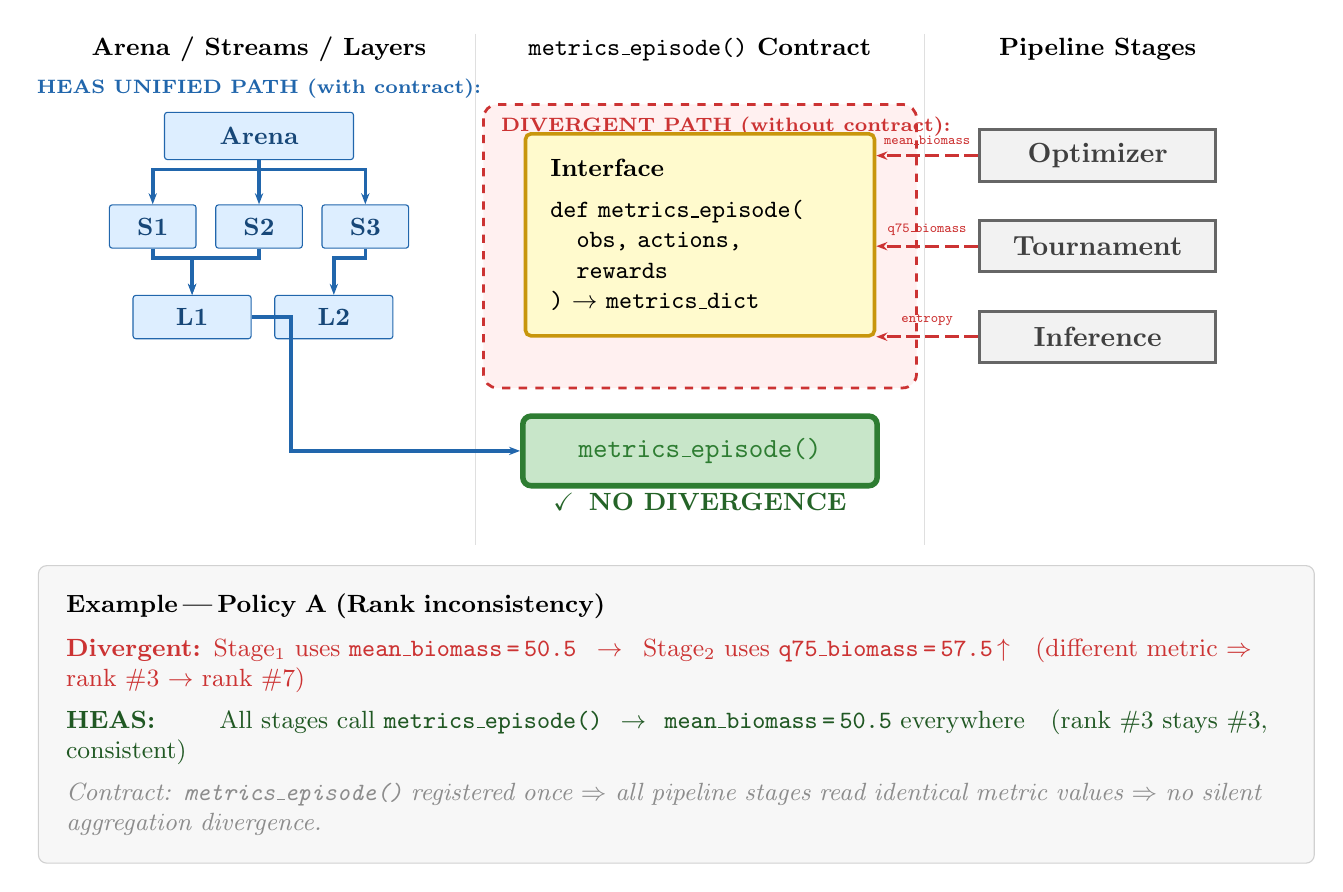
\begin{tikzpicture}[font=\small]

%% ══════════════════════════════════════════════════════════════════════════
%% COLUMN SEPARATORS & HEADERS
%% ══════════════════════════════════════════════════════════════════════════
\draw[gray!25, thin] (5.5, 9.4) -- (5.5, 2.9);
\draw[gray!25, thin] (11.2, 9.4) -- (11.2, 2.9);

\node[font=\small\bfseries] at (2.75, 9.2) {Arena / Streams / Layers};
\node[font=\small\bfseries] at (8.35, 9.2)  {\texttt{metrics\_episode()} Contract};
\node[font=\small\bfseries] at (13.4, 9.2)  {Pipeline Stages};


%% ══════════════════════════════════════════════════════════════════════════
%% LEFT COLUMN — HEAS Hierarchy
%% ══════════════════════════════════════════════════════════════════════════
\node[font=\scriptsize\bfseries, text=cBlue] at (2.75, 8.7)
  {HEAS UNIFIED PATH (with contract):};

%% Arena box
\node[
  draw=cBlue, fill=cBlueBg, rounded corners=1pt,
  minimum width=2.4cm, minimum height=0.6cm,
  font=\small\bfseries, text=cBlue!70!black, inner sep=5pt,
] (arena) at (2.75, 8.1) {Arena};

%% Stream boxes  S1 S2 S3
\node[draw=cBlue, fill=cBlueBg, rounded corners=1pt,
      minimum width=1.1cm, minimum height=0.55cm,
      font=\small\bfseries, text=cBlue!70!black, inner sep=4pt]
  (s1) at (1.4, 6.95) {S1};
\node[draw=cBlue, fill=cBlueBg, rounded corners=1pt,
      minimum width=1.1cm, minimum height=0.55cm,
      font=\small\bfseries, text=cBlue!70!black, inner sep=4pt]
  (s2) at (2.75, 6.95) {S2};
\node[draw=cBlue, fill=cBlueBg, rounded corners=1pt,
      minimum width=1.1cm, minimum height=0.55cm,
      font=\small\bfseries, text=cBlue!70!black, inner sep=4pt]
  (s3) at (4.1, 6.95) {S3};

%% Arena → S arrows
\draw[arrBlue] (arena.south) -- ++(0,-0.12) -| (s1.north);
\draw[arrBlue] (arena.south)                -- (s2.north);
\draw[arrBlue] (arena.south) -- ++(0,-0.12) -| (s3.north);

%% Layer boxes  L1 L2
\node[draw=cBlue, fill=cBlueBg, rounded corners=1pt,
      minimum width=1.5cm, minimum height=0.55cm,
      font=\small\bfseries, text=cBlue!70!black, inner sep=4pt]
  (l1) at (1.9, 5.8) {L1};
\node[draw=cBlue, fill=cBlueBg, rounded corners=1pt,
      minimum width=1.5cm, minimum height=0.55cm,
      font=\small\bfseries, text=cBlue!70!black, inner sep=4pt]
  (l2) at (3.7, 5.8) {L2};

%% S → L arrows
\draw[arrBlue] (s1.south) -- ++(0,-0.12) -| (l1.north);
\draw[arrBlue] (s2.south) -- ++(0,-0.12) -| (l1.north);
\draw[arrBlue] (s3.south) -- ++(0,-0.12) -| (l2.north);


%% ══════════════════════════════════════════════════════════════════════════
%% CENTRE COLUMN — Contract
%% ══════════════════════════════════════════════════════════════════════════

%% ── DIVERGENT PATH background (drawn first, behind nodes) ─────────────────
\begin{scope}[on background layer]
  \fill[cRedBg, rounded corners=5pt]   (5.6, 8.5) rectangle (11.1, 4.9);
  \draw[cRed, dashed, line width=1pt, rounded corners=5pt]
                                        (5.6, 8.5) rectangle (11.1, 4.9);
\end{scope}
\node[font=\scriptsize\bfseries, text=cRed, anchor=north west]
  at (5.7, 8.47) {DIVERGENT PATH (without contract):};

%% ── Interface box (yellow) ────────────────────────────────────────────────
\node[
  draw=cYellowBd, fill=cYellow, line width=1.3pt,
  rounded corners=2pt, inner sep=9pt,
  text width=3.8cm, align=left, anchor=north,
] (interface) at (8.35, 8.15) {
  \textbf{Interface}\\[4pt]
  \texttt{def metrics\_episode(}\\
  \texttt{\phantom{xx}obs, actions,}\\
  \texttt{\phantom{xx}rewards}\\
  \texttt{) $\to$ metrics\_dict}
};

%% ── metrics_episode() green box ───────────────────────────────────────────
\node[
  draw=cGreen, fill=cGreenBg, line width=2pt,
  rounded corners=3pt, inner sep=8pt,
  minimum width=4.5cm, minimum height=0.75cm,
  font=\normalsize\bfseries, text=cGreen,
] (contractNode) at (8.35, 4.1) {\texttt{metrics\_episode()}};

%% ── NO DIVERGENCE label ───────────────────────────────────────────────────
\node[font=\small\bfseries, text=cGreen!80!black]
  at (8.35, 3.45) {$\checkmark$\enspace NO DIVERGENCE};


%% ══════════════════════════════════════════════════════════════════════════
%% RIGHT COLUMN — Pipeline Stages
%% ══════════════════════════════════════════════════════════════════════════
\node[
  draw=cGrey, fill=cGreyBg, line width=1.1pt,
  minimum width=3.0cm, minimum height=0.65cm,
  font=\normalsize\bfseries, text=black!75, inner sep=5pt,
] (optimizer)  at (13.4, 7.85) {Optimizer};

\node[
  draw=cGrey, fill=cGreyBg, line width=1.1pt,
  minimum width=3.0cm, minimum height=0.65cm,
  font=\normalsize\bfseries, text=black!75, inner sep=5pt,
] (tournament) at (13.4, 6.7)  {Tournament};

\node[
  draw=cGrey, fill=cGreyBg, line width=1.1pt,
  minimum width=3.0cm, minimum height=0.65cm,
  font=\normalsize\bfseries, text=black!75, inner sep=5pt,
] (inference)  at (13.4, 5.55) {Inference};


%% ══════════════════════════════════════════════════════════════════════════
%% ARROWS
%% ══════════════════════════════════════════════════════════════════════════

%% Red dashed: Pipeline → Interface (each stage extracts its own metric)
\draw[arrRed] (optimizer.west)
  -- node[above, font=\tiny\ttfamily, text=cRed, midway] {mean\_biomass}
  (interface.east |- optimizer.west);

\draw[arrRed] (tournament.west)
  -- node[above, font=\tiny\ttfamily, text=cRed, midway] {q75\_biomass}
  (interface.east |- tournament.west);

\draw[arrRed] (inference.west)
  -- node[above, font=\tiny\ttfamily, text=cRed, midway] {entropy}
  (interface.east |- inference.west);

%% Blue: Left col → green contract box  (HEAS unified call)
\draw[arrBlue, line width=1.6pt]
  (l1.east) -- ++(0.5,0) |- (contractNode.west)
  node[midway, above, font=\tiny\itshape, text=cBlue, sloped] {};


%% ══════════════════════════════════════════════════════════════════════════
%% BOTTOM EXAMPLE STRIP
%% ══════════════════════════════════════════════════════════════════════════
\node[
  draw=black!18, fill=black!3,
  rounded corners=3pt, inner sep=10pt,
  text width=15.5cm, anchor=north,
] (example) at (8.05, 2.65) {
  \textbf{Example\,—\,Policy A\;\small(Rank inconsistency)}\\[5pt]
  \textcolor{cRed}{\textbf{Divergent:}\enspace
    Stage$_1$ uses \texttt{mean\_biomass\,=\,50.5}
    $\;\to\;$
    Stage$_2$ uses \texttt{q75\_biomass\,=\,57.5}\,$\uparrow$\quad
    {\small(different metric $\Rightarrow$ rank \#3 $\to$ rank \#7)}}\\[4pt]
  \textcolor{cGreen!70!black}{\textbf{HEAS:}\enspace\enspace\enspace\enspace\enspace
    All stages call \texttt{metrics\_episode()}
    $\;\to\;$
    \texttt{mean\_biomass\,=\,50.5} everywhere\quad
    {\small(rank \#3 stays \#3, consistent)}}\\[4pt]
  \textit{\textcolor{black!45}{%
    Contract: \texttt{metrics\_episode()} registered once
    $\Rightarrow$ all pipeline stages read identical metric values
    $\Rightarrow$ no silent aggregation divergence.}}
};

\end{tikzpicture}
\end{document}
